\documentclass[preprint, journal=prl]{revtex4-1}
\usepackage{graphicx}
\usepackage{amsmath}
\usepackage{braket}
\usepackage{float}
\usepackage{caption}
\usepackage{color}


\begin{document}
\title{Numerical Determination of the Hartree-Fock Stability of the Paramagnetic Electron Gas in 1, 2 and 3 Dimensions}
\author{Evan Curtin}
\author{So Hirata}
\email{Sohirata@illinois.edu}
\affiliation{Department of Chemistry, University of Illinois at Urbana-Champaign, 600 South Mathews Avenue, Urbana, Illinois 61801, USA}

\begin{abstract}
  In molecular electronic structure theory, breaking symmetry of a Hartree-Fock reference serves as a viable means to resolve spurious degeneracies in certain systems. This allows for the use of a wide array of post-Hartree-Fock methods to recover more of the correlation energy. While there exists proofs of the existence of lower energy broken symmetry solutions under certain circumstance in the finite case, we are unaware of analogous ones in the periodic case. This study presents numerical experiments into stability of paramagnetic solutions of the Homogeneous electron gas within the Hartree-Fock approximation to glean insight into the periodic case. We show that in 2 and 3 dimensions, the paramagnetic solution is unstable at $r_s$ above 0.87 and 3.2 bohr radii, respectively. In one dimension the solution is essentially always unstable, in agreement with Overhauser's theorem. This approach also lends itself to a means of finding lower energy broken symmetry solutions, at various levels of restriction within Hartree-Fock theory.
\end{abstract}

\maketitle

\section{Introduction} 
  Computational electronic structure in practice often requires a self-consistent solution to the Hartree-Fock equations. However, Being a solution to the HF equations ensures only that the solution is stationary with respect to the determined orbitals. If the solution is indeed a minimum, it is called ``stable'', while if there is any displacement in the electronic structure which lowers the energy, the solution is ``unstable''. A method for determining the stability of a Hartree-Fock solution was proposed by Thouless in 1960\cite{Thouless1960}. The condition was rederived into the expression familiar to quantum chemists by Čížek and Paldus in 1967\cite{Cizek1967}. Furthermore, the stability equations factorize depending on the symmetry of the Hartree-Fock eigenfunctions. To this end, Seeger and Pople outlined a hierarchical approach to systematically evaluate the stability of HF states in the restricted, unrestricted and generalized Hartree-Fock procedures\cite{Seeger1977}. Recently, the method has been used to aid the search for the lowest-energy Unrestricted Hartree-Fock (UHF) solutions in molecules, as well as the General Hartree-Fock (GHF) solutions in geometrically frustrated hydrogen rings which cannot conform even to the UHF scheme\cite{Pulay2016, Goings2015}. The lower energy HF solutions in these studies were located by first finding the instabilities in the higher spin-symmetry solutions, then using this information to obtain ``symmetry breaking'' displacements that lower the energy.    
    
  Previously it has been shown for finite systems with form-degenerate HOMO-LUMO, there always exists a symmetry-breaking instability, but this theorem does not hold in the infinite case \cite{Yamada2015}. To investigate HF instabilities in zero band gap solids, a natural starting point is the Homogeneous Electron Gas (HEG, often called Jellium or Uniform Electron Gas) model. The model consists of electrons in a box with periodic boundary conditions  and the constraint that the entire system is charge-neutral via a uniform background positive  charge. The resulting Coulomb interactions cancel exactly, and the only remaining terms are due   to kinetic and exchange energies. Historically it was thought that the plane-wave paramagnetic solution to the HF equations for this model was the ``correct'' solution. However, in a landmark paper, Overhauser showed that certain symmetry broken solutions \emph{always} have lower-energy than the paramagnetic solutions at all electron densities\cite{Overhauser1962}. This hints at, but does not show, that the analogous triplet instability theorem persists in the infinite case.  
        
  Overhausers' paper sparked new interest in the HEG, and since then Energies of various phases thereof have been computed to great accuracy\cite{Ceperley1980}. More recently, phase diagrams have been determined for the HEG in 2 and 3 dimensions\cite{Delyon2008, Bernu2011, Baguet2013}. In all cases the phase diagrams are made by computing the energies of the polarized and unpolarized states, and comparing them. This approach necessitates that the form of the solutions is known ahead of time. 
  
  The present work focuses on directly calculating the Hartree-Fock stability of the paramagnetic homogeneous electron gas as a function of electron density in order to see if the singlet/instability theorems apply in this continuous system.  It is important here to note that instability is a sufficient but not necessary condition for the presence of a lower energy solution, and therefore Overhauser's theorem does not strictly imply instability at all densities. Given this fact, we can learn about the differences between instability detection and direct minimization techniques within Hartree-Fock theory. It may also be insightful to see if the difference depend on the level of restriction used in the HF equations (i.e. UHF vs GHF).  
        
\section{Method}

  Usually to find a symmetry-broken HF solution of lower energy, the method employed is to determine the stability of a found Hartree-Fock solution. Instabilities are indicated by a negative eigenvalue in the Electronic Hessian, 
  \begin{equation}
    \bf{H}=
    \begin{bmatrix}
      \bf{A} &\bf{B} \\
      \bf{B}^* & \bf{A}^* \\
    \end{bmatrix},
  \end{equation} 
  where the matrices $\mathbf{A}$ and $\mathbf{B}$ have dimension $N_{occupied} \times N_{virtual}$ with elements given by
  \begin{align}
     A_{i \rightarrow a, j \rightarrow b} &= (\epsilon_a-\epsilon_i)\delta_{ij}\delta_{ab} 
     + \left< aj||ib \right>, \\
     B_{i \rightarrow a, j \rightarrow b} &= \left< ab||ij \right>. 
  \end{align}    
  
  Where occupied states are labelled by $i$ and $j$, virtual by $a$ and $b$, and $i \rightarrow a$ refers to the excitation which replaces state $i$ with state $a$. The relevant two electron notation is
  \begin{equation}
    \left< pq||rs \right> = \left< pq|rs \right> - \left< pq|sr \right>,
  \end{equation}
  where, 
  \begin{equation}
    \left< pq|rs \right> = 
    \int \int \phi^*_p(\vec{x}_1) \phi^*_q(\vec{x}_2) 
    V(\vec{r}_1, \vec{r}_2) 
    \phi_r(\vec{x}_1) \phi_s(\vec{x}_2) 
    d\vec{x_1} d\vec{x_2}, 
  \end{equation}
  and states labeled with $p$, $q$, $r$, or $s$ are either occupied or virtual. In this paper angled brackets $\left< ... \right>$ denote integrals over spatial and spin degrees of freedom $d\vec{x}$, while parentheses $\left ( ... \right ) $ denote integration over spatial coordinates, $d\vec{r}$, only. For a paramagnetic HF solution (RHF), integrating the Orbital Hessian elements over spin yields the singlet and triplet instability matrices ($\bf{{}^1H}$ and $\bf{{}^3H}$, respectively)\cite{Dunning1967,Seeger1977}.
  \begin{subequations}
    \begin{eqnarray}
      {}^{1}{A'}_{i\rightarrow a, j\rightarrow b} &=& 
      (\epsilon_a-\epsilon_i)\delta_{ij}\delta_{ab} 
      + 2\left(aj|ib\right)-\left(aj|bi\right)\\
      {}^{3}{A'}_{i\rightarrow a, j\rightarrow b} &=& 
      (\epsilon_a-\epsilon_i)\delta_{ij}\delta_{ab} 
      - \left(aj|bi\right)\\
      {}^{1}{B'}_{i\rightarrow a, j\rightarrow b} &=& 2\left(ab|ij\right) - \left(ab|ji\right)\\
      {}^{3}{B'}_{i\rightarrow a, j\rightarrow b} &=& -\left(ab|ji\right)
    \end{eqnarray}
  \end{subequations}
  The lowest eigenvalue of both of these matrices will reveal the stability of the RHF solution. If  ${}^1\bf{H}$ has negative eigenvalues, the solution is unstable with respect to changes that preserve singlet character (singlet instability), while if ${}^3\bf{H}$ has negative eigenvalues, the solution is unstable towards displacements that would change the wavefunction towards a triplet state (triplet instability). The solution is stable if neither ${}^1\bf{H}$ nor ${}^3\bf{H}$ has a negative eigenvalue. An eigenvalue of 0 does not indicate instability, and this case is discussed in detail by Cui et al \cite{Cui2013}.   
    	
  To apply the stability analysis to the electron gas, start with the Jellium Hamiltonian in atomic units, 
  \begin{equation}\label{hamiltonian}
   	\hat{H} = - \sum_i \frac{\hat{p}_i^2}{2}  + \sum_{i < j} V(\vec{r}_i, \vec{r}_j)  .
  \end{equation}
  One solution to the Hartree-Fock equations in $D$ dimensions are plane waves of the form	
  \begin{equation}\label{planewave}
   	\phi_{\vec{k}} =
    \frac{1} { \sqrt{L ^ D} } e ^ {i \vec{k} \cdot \vec{x}},
  \end{equation}
  where $L$ is the length of one side of the direct lattice with cubic symmetry. Using this as the basis for the rest of the analysis, the two electron repulsion integrals are analytic and  well-behaved in two and three dimensions\cite{Delyon2008, Guiliani2005}
  \begin{align}
    \left( \vec{k}, \vec{k}' | \vec{k}'', \vec{k}''' \right) 
    \stackrel{ \text{2D, 3D} }{=}&
    \begin{cases} 
      \frac{\pi} {L ^ D} \frac{ 2^{D-1} } { | \vec{k} - \vec{k}'' | ^ {D-1} } 
      & \vec{k}''' = \vec{k} + \vec{k}' - \vec{k}'' + n\vec{G} \textbf{ and } | \vec{k} - 
      \vec{k}''| \neq 0 \\
      0 
      & \text{else},
    \end{cases}
  \end{align}
  where $n\vec{G}$ is any integer times a reciprocal lattice vector of the system. The orbital energies are
  \begin{equation}\label{eq:hf_orb_energy}
    \epsilon_{\vec{k},\sigma}=
    \frac{\hbar^2\vec{k}^2}{2m} - \sum\limits_{\vec{k}}^{|\vec{k}|< 
    k_f}n_{\vec{k}\sigma} \left( \vec{k}, \vec{k}' |\vec{k}', \vec{k} \right),
  \end{equation}
  where $n_{\vec{k}\sigma}$ is the occupation number of the state with momentum $\vec{k}$ and spin $\sigma$ \cite{Guiliani2005}. In one dimension, the two electron integral diverges, and it is common to use a delta function interaction, 
  \begin{equation}
    V(r_{12}) = V_0\delta(r_{12}),
  \end{equation}
  and the two electron integral in this case is simply
  \begin{align}\label{eq:ERI_1d}
    \braket{\vec{k}, \vec{k}' | \vec{k}'', \vec{k}'''} 
    \stackrel{ \text{1D} }{=}&
    \begin{cases} 
      \frac{V_0}{L} 
      & \vec{k}''' = \vec{k} + \vec{k}' - \vec{k}'' + n\vec{G}\\
      0 
      & \text{else}.
    \end{cases}
  \end{align}  
  These expressions can be used to evaluate the stability of the paramagnetic electron gas. In doing so, presence of instabilities of triplet (${}^3\mathbf{H}$) character are a sufficient, but not necessary, condition that a solution with different densities of $\alpha$ and $\beta$ spin exists which has lower energy than the paramagnetic solution. An example of such a solution would be the spin-density-wave (SDW) solution. 
   
\section{Results}   
  Using the equations for energies and two electron integrals, the stability analysis was performed on the paramagnetic HEG model as a function of electron density (or equivalently, the Wigner-Seitz radius, $r_s$). The approach of explicitly constructing and diagonalizing the orbital hessian is intractable both in terms of memory and calculation time requirements. Since the instability condition is that the any eigenvalue is negative, it suffices to calculate the sign of only the lowest eigenvalue. This is a task well suited for an iterative subspace solver. To this end, the Jacobi-Davidson algorithm was from the SLEPc library was used to calculated the lowest eigenvalues using the Blue Waters Supercomputer\cite{Hernandez2005}. 
  
  A basis of plane waves with simple cubic symmetry was used for all calculations, and the number of k-points was incremented until the lowest eigenvalues were sufficiently converged {\color{red} (for 1D and 2D more data can be gathered but in 3D getting more data is computationally unfeasible at the moment)}. In the 1D calculations, a potential of $V_0 = 1$ in atomic units was used.
  \begin{figure}[H]
    \centering
    \includegraphics[]{fit_curves.eps}
    \caption{The lowest eigenvalue of ${}^1\mathbf{H}$ (Singlet instability) and ${}^3\mathbf{H}$ (Triplet instability) as a function of $r_s$ for a representative calculation in 2 dimensions with 1936 k-points.}
    \label{fig:singlet_convergence}
  \end{figure}
  \begin{figure}[H]
    \centering
    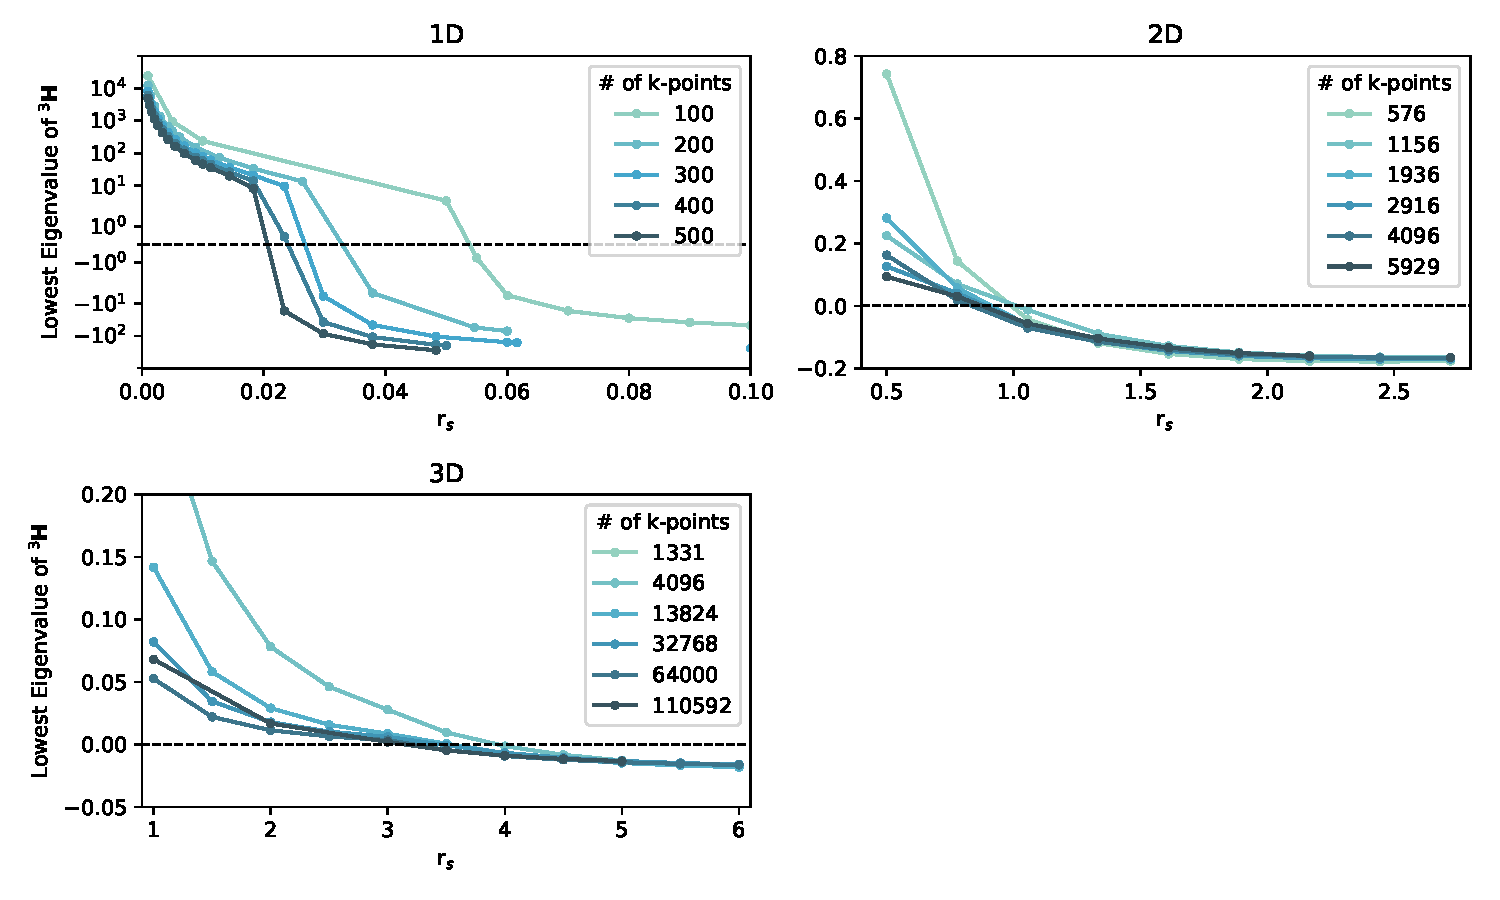
\includegraphics[width=\textwidth]{../../images/triplet-stability-convergence.pdf}
    \caption{The lowest eigenvalue of ${}^3\mathbf{H}$ as a function of $r_s$ with increasing number of k-points in 1, 2 and 3 dimensions.}
    \label{fig:triplet_convergence}
  \end{figure}
  To determine the $r_s$ at which the lowest eigenvalue of $\mathbf{H}$ changes sign, the lowest eigenvalues were linearly interpolated  as a function of $r_s$ and solving
  \begin{equation} \label{eq:transition_rs}
    \lambda_{min}(r_s) = 0.
  \end{equation}
  The solution to eq. \ref{eq:transition_rs} is referred to as the transition $r_s$ and this quantity was determined while increasing the number of k-points in the simulation to convergence (see Fig. \ref{fig:onset}).
  \begin{figure}[H]
    \centering
    \includegraphics[width=\textwidth]{onsets.eps}
    \caption{The value of $r_s$ at which the singlet (green) and triplet (blue) instability    occurs with increasing number of k-points in 1, 2 and 3 dimensions. In the 1D case (left), the singlet instability never appeared in the calculations performed. }
    \label{fig:onset}
  \end{figure}
  
  
  \begin{table}[H]
  \centering
  \caption{Critical values of $r_s$.}
    \begin{tabular}{ c  c  c }
      D~ & ~ Instability (bohr$^{-1}$) ~ &  \\ 
      \hline
      1    &  0.51 &  \\
      2    &  0.86 & 0.8 \\
      3    &  2.92 & 3.0 \\
      \hline
     \end{tabular}
  \label{table:transition_rs}
  \end{table}  
  The transition $r_s$ values are presented in table \ref{table:transition_rs}. These results are consistent with those seen by other methods, which show the emergence of broken symmetry phases with distinguishably lower energy at $r_s \approx 0.8$ in 2D and $r_s \approx 3$ in 3D\cite{Baguet2014, Bernu2011}. On the other hand, the transition $r_s$ for one dimension tends towards zero and stays quite close as the number of grid points increases. 

  
\section{Conclusion}
  

  
\begin{acknowledgements}
The authors would like to thank...
\end{acknowledgements}

\section{References}
\bibliography{references}

\end{document}